\documentclass[draft,final]{thesisclass} % Remove option 'final' to obtain debug information.

% Load packages to allow in- and output of non-ASCII characters.
\usepackage{lmodern}        % Use an extension of the original Computer Modern font to minimize the use of bitmapped letters.
\usepackage[T1]{fontenc}    % Determines font encoding of the output. Font packages have to be included before this line.
\usepackage[utf8]{inputenc} % Determines encoding of the input. All input files have to use UTF8 encoding.

% Extended LaTeX functionality is enables by including packages with \usepackage{...}.
\usepackage{amsmath}    % Extended typesetting of mathematical expression.
\usepackage{amssymb}    % Provides a multitude of mathematical symbols.
\usepackage{mathtools}  % Further extensions of mathematical typesetting.
\usepackage{microtype}  % Small-scale typographic enhancements.
\usepackage[inline]{enumitem} % User control over the layout of lists (itemize, enumerate, description).
\usepackage{multirow}   % Allows table elements to span several rows.
\usepackage{booktabs}   % Improves the typesetting of tables.
\usepackage{subcaption} % Allows the use of subfigures and enables their referencing.
\usepackage[ruled,linesnumbered,algochapter]{algorithm2e} % Enables the writing of pseudo code.
\usepackage[usenames,dvipsnames,table]{xcolor} % Allows the definition and use of colors. This package has to be included before tikz.
\usepackage{nag}       % Issues warnings when best practices in writing LaTeX documents are violated.
\usepackage{todonotes} % Provides tooltip-like todo notes.
\usepackage{hyperref}  % Enables hyperlinking in the electronic document version. This package has to be included second to last.
\usepackage[acronym,toc]{glossaries} % Enables the generation of glossaries and lists of acronyms. This package has to be included last.
\usepackage{lipsum}  % Provides blind text.
\usepackage{acronym} % Provides a list of acronyms.
\usepackage{float} % Provides the H float modifier option.

% Define convenience functions to use the author name and the thesis title in the PDF document properties.
\newcommand{\authorname}{Hannes Brantner} % The author name without titles.
\newcommand{\thesistitle}{Enhancing recruitment efficiency by exploring the impact of large language models on optimizing the identification of qualified applicants} % The title of the thesis. The English version should be used, if it exists.

% Set PDF document properties
\hypersetup{
    pdfpagelayout   = TwoPageRight,           % How the document is shown in PDF viewers (optional).
    linkbordercolor = {Melon},                % The color of the borders of boxes around hyperlinks (optional).
    pdfauthor       = {\authorname},          % The author's name in the document properties (optional).
    pdftitle        = {\thesistitle},         % The document's title in the document properties (optional).
    pdfsubject      = {LLMs in HR},              % The document's subject in the document properties (optional).
    pdfkeywords     = {Machine Learning, HR, Human Resources, AI, LLM} % The document's keywords in the document properties (optional).
}

\setpnumwidth{2.5em}        % Avoid overfull hboxes in the table of contents (see memoir manual).
\setsecnumdepth{subsection} % Enumerate subsections.

\nonzeroparskip             % Create space between paragraphs (optional).
\setlength{\parindent}{0pt} % Remove paragraph indentation (optional).

\makeindex      % Use an optional index.
\makeglossaries % Use an optional glossary.
%\glstocfalse   % Remove the glossaries from the table of contents.

% Set persons with 4 arguments:
%  {title before name}{name}{title after name}{gender}
%  where both titles are optional (i.e. can be given as empty brackets {}).
\setauthor{Ing. Dipl.-Ing.}{\authorname}{BSc}{male}
\setadvisor{}{Michaela Wawra}{MSc}{female}

% For bachelor and master theses:
% \setfirstassistant{Pretitle}{Forename Surname}{Posttitle}{male}
% \setsecondassistant{Pretitle}{Forename Surname}{Posttitle}{male}
% \setthirdassistant{Pretitle}{Forename Surname}{Posttitle}{male}

% For dissertations:
% \setfirstreviewer{Pretitle}{Forename Surname}{Posttitle}{male}
% \setsecondreviewer{Pretitle}{Forename Surname}{Posttitle}{male}

% For dissertations at the PhD School and optionally for dissertations:
% \setsecondadvisor{Pretitle}{Forename Surname}{Posttitle}{male} % Comment to remove.

% Required data.
\setregnumber{01614466}
\setdate{01}{10}{2023} % Set date with 3 arguments: {day}{month}{year}.
\settitle{\thesistitle}{\thesistitle} % Sets English and German version of the title (both can be English or German). If your title contains commas, enclose it with additional curvy brackets (i.e., {{your title}}) or define it as a macro as done with \thesistitle.
\setsubtitle{}{} % Sets English and German version of the subtitle (both can be English or German).

% Select the thesis type: bachelor / master / doctor.
% Bachelor:
% \setthesis{bachelor}
%
% Master:
\setthesis{master}
\setmasterdegree{master} % dipl. / rer.nat. / rer.soc.oec. / master
%
% Doctor:
%\setthesis{doctor}
%\setdoctordegree{rer.soc.oec.}% rer.nat. / techn. / rer.soc.oec.

% For bachelor and master:
\setcurriculum{Master in Business Administration (One Year MBA)}{Master in Business Administration (One Year MBA)} % Sets the English and German name of the curriculum.

% Optional reviewer data:
\setfirstreviewerdata{Affiliation, Country}
\setsecondreviewerdata{Affiliation, Country}

% Add glossary entries.
\newglossaryentry{LLM}
{
    name=Large Language Model,
    description={A Large Language Model is reading and emitting text, enabling it to perform tasks such as translation, summarization, and question answering.}
}

\begin{document}

\frontmatter % Switches to roman numbering.
% The structure of the thesis has to conform to the guidelines at
%  https://informatics.tuwien.ac.at/study-services

% \addtitlepage{naustrian} % German title page.
\addtitlepage{english} % English title page.
\addstatementpage

% citation tutorial
% cite only page 1
% \cite[1]{discrimination_algorithms} \newline
% cite page 2 to 5
% \cite[2-5]{discrimination_algorithms} \newline
% cite page 3 and the following page
% \cite[3f]{discrimination_algorithms} \newline
% cite page 3 and the following pages
% \cite[3ff]{discrimination_algorithms} \newline

\begin{acknowledgements*}
\lipsum[2-4]
\end{acknowledgements*}

\begin{abstract}
\lipsum[2-4]
\end{abstract}

% Select the language of the thesis, e.g., english or naustrian.
\selectlanguage{english}

% Add a table of contents (toc).
\tableofcontents % Starred version, i.e., \tableofcontents*, removes the self-entry.

% Switch to arabic numbering and start the enumeration of chapters in the table of content.
\mainmatter

\chapter{Introduction}

\section{Background}
\subsection{Large Language Models}
The machine learning model type \gls{LLM} is commonly abbreviated as \acs{LLM} and makes natural language texts processable for computers.
The model works by compressing the read text into an internal state and based on this state an output text is generated.
As the model compresses the data according to the learned patterns in the training data, it does not understand the text in the same way as humans do.
These models are used to perform tasks such as translation, summarization, and question answering \cite[1]{llm_literature_review}.
As this enabled a wide field of automization for application fields that were primarily carried out by humans, many technology companies have developed their own \acs{LLM} and made their services available to the public while keeping their source code mostly private.
Some notable example are the PaLM 2 model by Google \cite{palm2} that powers Bard, the GPT-4 model by OpenAI \cite{gpt4} that powers ChatGPT and the Llama 2 model by Meta \cite{llama2}.
The Llama 2 model is the only model from the picked three candidates that has been released with public source code.
That means that researches and engineers around the world can use the model as building block and either improve the underlying mechanisms or try to incorporate it in their own applications.
The real breakthrough of \acs{LLM}s came with the release of the GPT-3 model by OpenAI \cite{gpt3} that powered the initial version of ChatGPT.
They offered the model's capabilities as a website that was accessible to the public and allowed users to insert text and receive a response from the model.
As described in \cite[1]{gpt3}, the model provided very good performance on various \acs{NLP} datasets that include tasks like translation and question answering.
To briefly visualize the complexity behind a \acs{LLM}, consider the function $f_{a,b,c}(x) = ax^2+bx+c$ that has the three parameters $a$, $b$ and $c$.
Here, the function $f$ maps the input data denoted as $x$ to the output data denoted as $f(x)$.
The input data in the \acs{NLP} case is the input text and the output data is the output text.
\acs{LLM}s also make use of parameterized and differentiable functions in their internal structure to map the input text to the output text, but they have orders of magnitudes more parameters than this sample function.
For example, the model GPT-3 uses 175 billion parameters \cite[1]{gpt3} in total. The parameter count of GPT-4 was not disclosed in their technical report \cite{gpt4}.
The training data needed to train these models was present in the required amounts because the researchers have not used reinforcement learning \cite{rl_bible} or supervised learing \cite[3]{sl_bible}.
Reinforcement learning gives the model a reward when an action was good and a punishment when an action was bad, this can be done by letting the model train in the real world which has bad scalability or in simulators that must be coded to mimic the real world which is also a very difficult and time consuming task.
For example, animals learn that behaviors that lead to food are good and behaviors that lead to hunger are bad.
The supervised learning approach labels input data with the desired output label and based on these mappings and a huge amount of training samples, the model will adjust its parameters to map the input data correctly.
An example would be input images that would be labeled with the object that can be seen on the images. So each input image must be labeled by hand before the model can be trained to predict it itself correctly.
To compress the patterns in the training data and fill them into the model parameters, huge amounts of training data are needed as the parameter count of \acs{LLM}s is huge.
Both techniques were not sufficient to train models of that sheer size, so the researchers used a technique called self-supervised learning \cite[7]{llm_literature_review} where the model tries to fill in artificially generated gaps in the text.
Because the gaps are artificially introduced, the expected output is known in advance, so the model can be trained without the need of labeled training data which makes this technique immensly scalable.
Before the text is fed to the model it is tokenized \cite[4]{llm_literature_review}, that means the text is converted into a sequence of tokens which can either be symbols, characters, subwords and words.
The model gets the tokenized text input and predicts the follow-up output tokens that will likely follow these input tokens. The output tokens are converted back into text and then the text from the artifical gap is compared to the model output.
Based on this comparison, the model parameters are adjusted. As no human data labelling or costly real-world or simulator training is needed, the model can be trained on huge amounts of data.
Most of the text data used for training large language models is scraped from the internet \cite[1]{llm_literature_review}.
The context size of a \acs{LLM} is the number of tokens that the model can store in its internal state while generating the output tokens, so it is the history of tokens it can access while generating the response.
For example, the context size of the Llama 2 model is 4096 tokens \cite[47]{llama2}.
The tokenizer that OpenAI is using, can be accessed via this website \cite{openai_tokenizer}.
The output tokens of a \acs{LLM} are generated token by token, so when the first token is generated, it is appended to the input and the model generates the next token based on the input that now contains the first generated token. Afterwards, it is run iteratively in the same way.
That means that the total output token size is also constrained by the context size, when the full history of tokens should be within the context size while generating the output.
The model stops the output loop, when the model emits the stop token. That means that it has finished the output token generation.
Most of \acs{LLM}s are based on the machine learning model type called Transformers \cite[1]{transformer} which is a neural network architecture that is based on the attention mechanism.

\section{Problem Statement}
As described in \cite[1]{ai_recruiting}, the the average firm's value by 2000 was roughly consisting of 65\% of value from intangible assets.
This has evolved a lot, as by the end of 1980, around 70 to 90\% of tangible assets were accountable for the average firm's value \cite[1]{ai_recruiting}.
This means that the value of a firm is more and more dependent on the quality of its employees and the knowledge they possess and this ongoing process does not seem to come to a hault in the near future.
The technological context of how companies recruit people has also evolved a lot over the last decades, as machine learning tools are more and more used to automate processes or assist humans in attracting the right candidates, screening, assessing and selecting them \cite[2]{ai_recruiting}.
The article \cite[2-4]{ai_recruiting} described four evolution stages of recruting which are the following:
\begin{enumerate}
    \item \textbf{Analog Recruiting}\\
    The first stage is the analog recruiting stage where people were the main mechanism of recruiting new employees.
    Prospective applicants needed to go to the company to manually turn a paper job application in.
    Companies want to maximze the information richness they supply for the current job vacancy but also the information reach to attract as many promising applicants as possible.
    But as described in \cite[2]{ai_recruiting}, in analog recruting this two goals faced the analog reach and richness frontier as shown in \ref{fig:analog_reach_richness_frontier}:
    \begin{figure}[H]
        \centering
        \includegraphics[scale=0.7,page=2,width=0.6\linewidth,trim={300 100 55 515},clip]{literature/ai_recruiting.pdf}
        \caption{Analog reach and richness frontier \cite[2]{ai_recruiting}}
        \label{fig:analog_reach_richness_frontier}
    \end{figure}
    \item \textbf{Digital Recruting 1.0}
    \item \textbf{Digital Recruting 2.0}
    \item \textbf{Digital Recruting 3.0}
\end{enumerate}


\section{Research Objectives}
\lipsum[2-4]

\section{Research Question}
\lipsum[2-4]

\section{Significance}
\lipsum[2-4]

\section{Scope and Limitations}
\lipsum[2-4]

\chapter{Methodology}

\section{Research Design}
\lipsum[2-4]

\section{Data Collection}
\lipsum[2-4]

\section{Data Analysis}
\lipsum[2-4]

\chapter{Implementation}

\section{Input Data Preprocessing}
\lipsum[2-4]

\section{Prompt Design}
\lipsum[2-4]

\section{Output Data Postprocessing}
\lipsum[2-4]

\chapter{Results}

\section{Data Overview}
\lipsum[2-4]

\section{Machine Learning Impact Analysis}
\lipsum[2-4]

\section{Visualizations}
\lipsum[2-4]

\chapter{Discussion}

\section{Interpretation}
\lipsum[2-4]

\section{Comparison}
\lipsum[2-4]

\section{Machine Learning Benefits}
\lipsum[2-4]

\section{Challenges and Ethical Considerations}
\lipsum[2-4]

\section{Future Implications}
\lipsum[2-4]

\chapter{Conclusion}

\section{Summary}
\lipsum[2-4]

\section{Contributions}
\lipsum[2-4]

\section{Practical Implications}
\lipsum[2-4]

\section{Limitations}
\lipsum[2-4]

\section{Final Thoughts}
\lipsum[2-4]

\backmatter

% Use an optional list of figures.
\listoffigures % Starred version, i.e., \listoffigures*, removes the toc entry.

% Use an optional list of tables.
\cleardoublepage % Start list of tables on the next empty right hand page.
\listoftables % Starred version, i.e., \listoftables*, removes the toc entry.

% Use an optional list of alogrithms.
% \listofalgorithms
% \addcontentsline{toc}{chapter}{List of Algorithms}

% Add an index.
\printindex

% Add a glossary.
\printglossaries

% Add acronym entries.
\begin{acronym}
    \acro{LLM}{Large Language Model}
    \acro{NLP}{Natural Language Processing}
\end{acronym}

% Add a bibliography.
% comment out when finished
\nocite{*}
\bibliographystyle{apalike}
\bibliography{thesis}

\end{document}